\documentclass{beamer}
\usepackage[utf8]{inputenc}
\usepackage[english,russian]{babel}
\usepackage{amsmath,mathrsfs,mathtext}
\usepackage{graphicx,epsfig}
\usepackage{caption}
\usepackage{subfig}
\usepackage{bm}
\usetheme{Warsaw}%{Singapore}%{Warsaw}%{Warsaw}%{Darmstadt}
\usecolortheme{sidebartab}
%\definecolor{beamer@blendedblue}{RGB}{15,120,80}

\newcommand{\T}{^{\mathsf{T}}}
\DeclareMathOperator*{\argmax}{arg\,max}  % in your preamble
\DeclareMathOperator*{\argmin}{arg\,min}  % in your preamble 

\graphicspath{{../figures}, {../figures_delta}}

%\usepackage{biblatex}
\usepackage{hyperref}
\renewcommand{\thefootnote}{\arabic{footnote}}

%----------------------------------------------------------------------------------------------------------
\title[\hbox to 56mm{Восстановление снимков фМРТ \hfill\insertframenumber\,/\,\inserttotalframenumber}]
{Восстановление снимков фМРТ \\ по просматриваемому видеоряду}
\author[Н.\,С.~Киселев]{\large Никита Сергеевич Киселев}
\institute{\large
Московский физико-технический институт\par
(национальный исследовательский университет)}

\date{\footnotesize{\emph{Курс:} Автоматизация научных исследований\par (Моя первая научная статья)/Группа 003, весна 2023 \\
\par\emph{Эксперт:} А.\,В.~Грабовой
}}
%----------------------------------------------------------------------------------------------------------
\begin{document}
%----------------------------------------------------------------------------------------------------------
\begin{frame}
%\thispagestyle{empty}
\titlepage
\end{frame}
%-----------------------------------------------------------------------------------------------------
\begin{frame}{Цель исследования}
    \begin{block}{Проблема}
        Аппроксимация показаний датчиков фМРТ при взаимодействии человека с внешним миром.
    \end{block}
    \begin{block}{Цель}
        Аппроксимация последовательности снимков фМРТ по видеоряду,
	    просматриваемому человеком.
    \end{block}
    \begin{block}{Предлагается}
        \begin{enumerate}
            \item Восстановление изменения снимка фМРТ с учетом времени задержки $\Delta t$.
            \item Исследование свойств построенного метода и проверка гипотез.
        \end{enumerate}
    \end{block}
\end{frame}
%----------------------------------------------------------------------------------------------------------
\begin{frame}{Постановка задачи}
    \begin{figure}[h!]
        \centering
        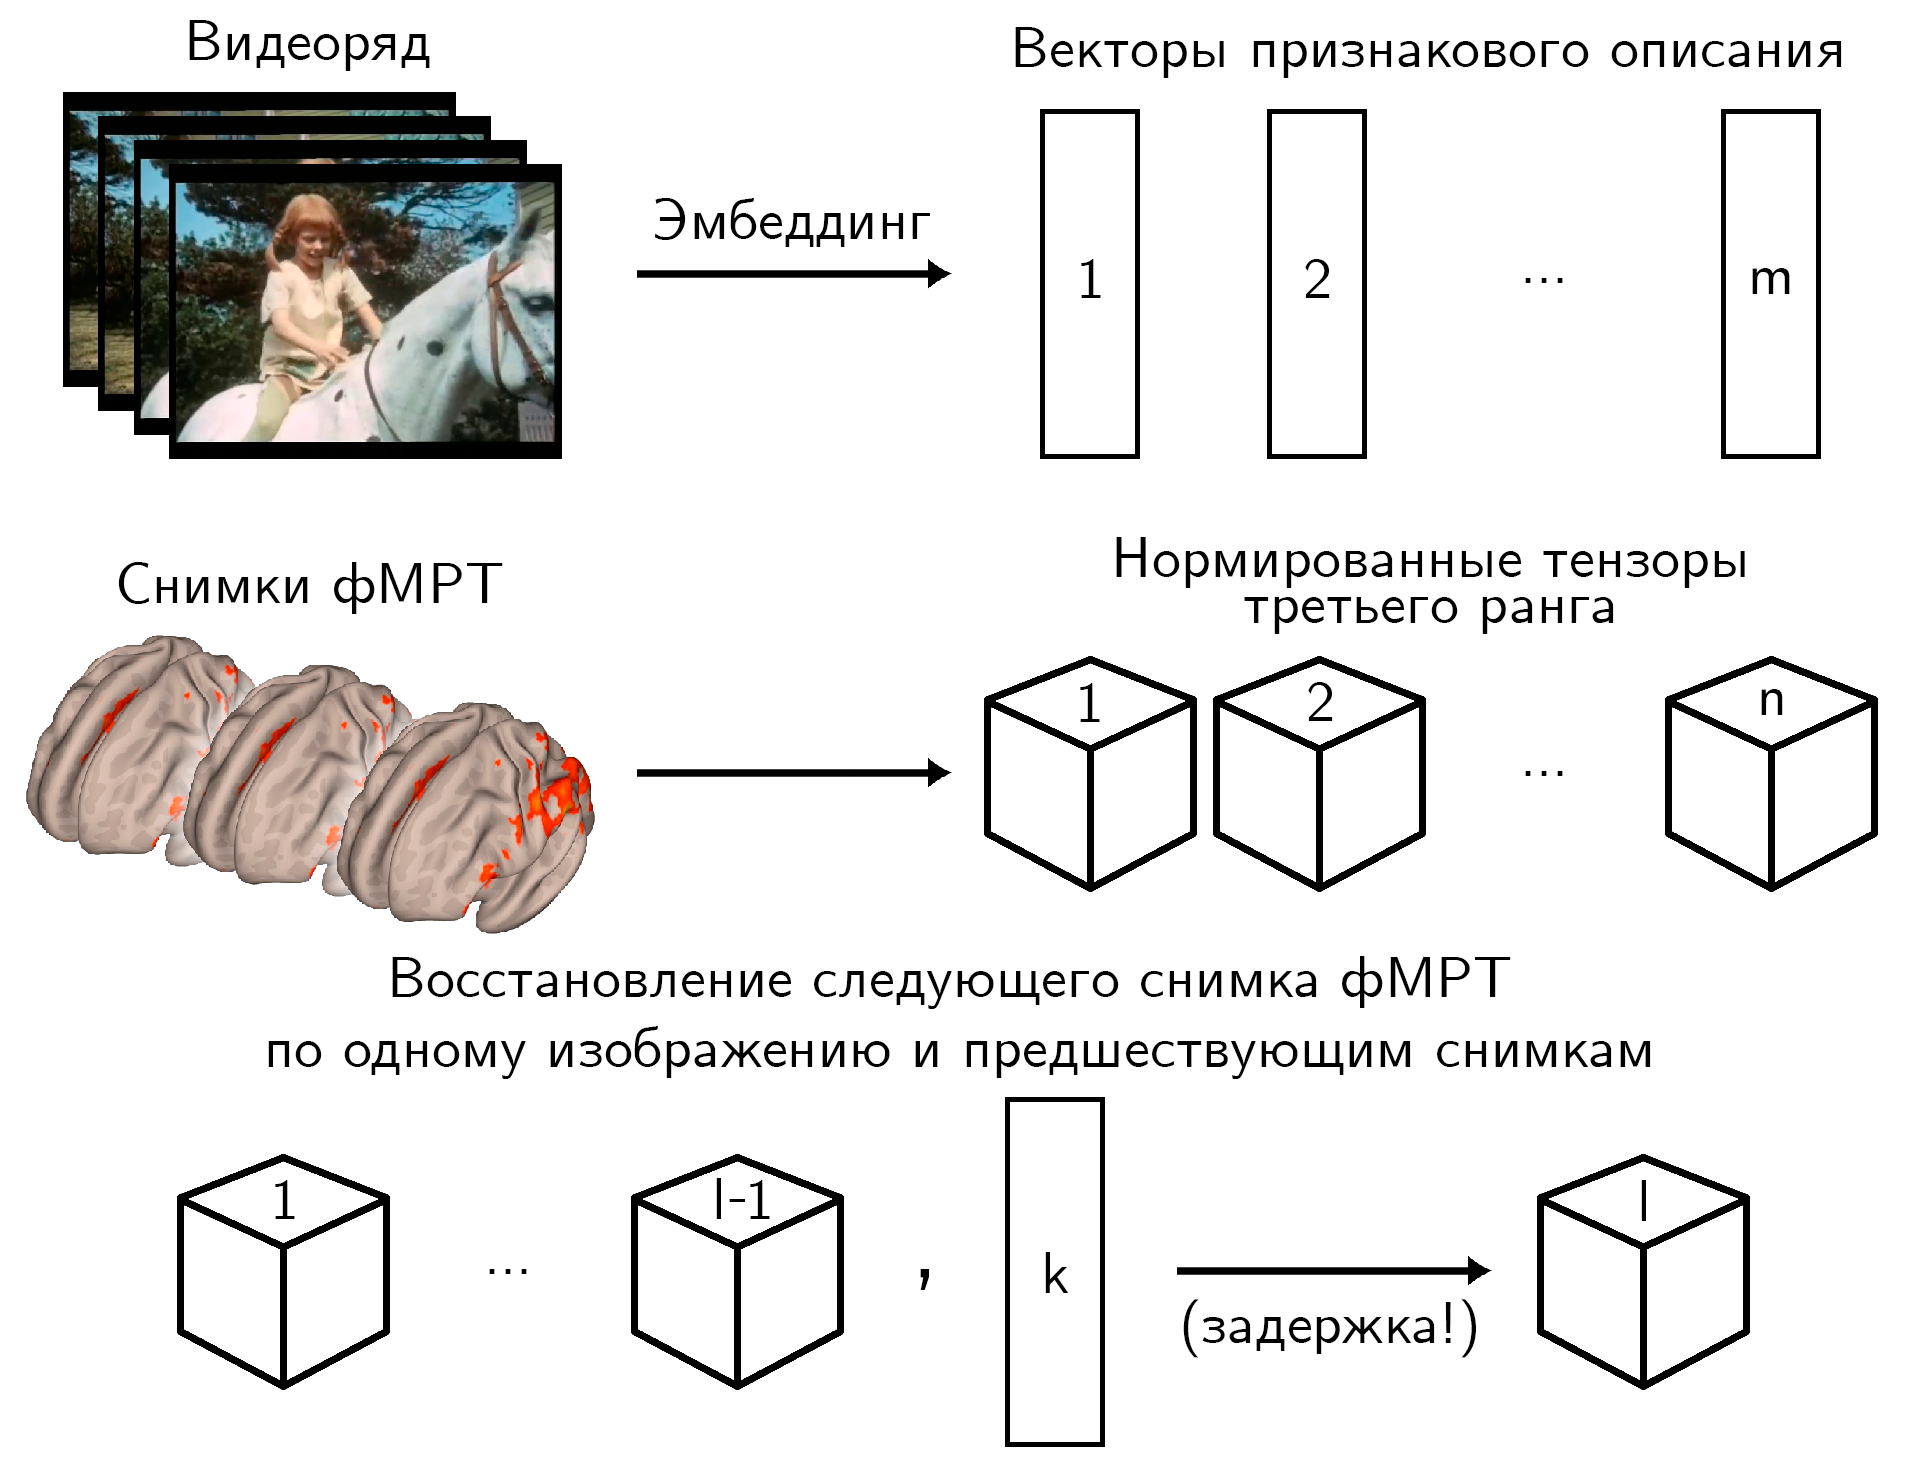
\includegraphics[width=\textwidth]{scheme.png}
    \end{figure}
\end{frame}
%----------------------------------------------------------------------------------------------------------
\begin{frame}{Постановка задачи}
    Пусть задана частота кадров $\nu \in \mathbb{R}$ и продолжительность $t \in \mathbb{R}$ видеоряда. 
	Задан видеоряд
	\begin{equation*}
		\label{eq1}
		\mathbf{P} = [\mathbf{p}_1, \ldots, \mathbf{p}_{\nu t}], \quad\
		\mathbf{p}_{\ell} \in \mathbb{R}^{W \times H \times C}.
	\end{equation*}

	Обозначим частоту снимков фМРТ $\mu \in \mathbb{R}$. Задана последовательность снимков 
	\begin{equation*}
		\label{eq2}
		\mathbf{S} = [\mathbf{s}_1, \ldots, \mathbf{s}_{\mu t}], \quad\
		\mathbf{s}_{\ell} \in \mathbb{R}^{X \times Y \times Z}.
	\end{equation*}

	Необходимо построить отображение
    \begin{block}{}
        \begin{equation*}
            \label{eq3}
            \mathbf{g}(\mathbf{p}_1, \ldots, \mathbf{p}_{k_{\ell} - \nu \Delta t}; \mathbf{s}_1, \ldots, \mathbf{s}_{\ell-1}) = \mathbf{s}_{\ell},
        \end{equation*}
        \begin{equation*}
            \label{eq4}
            \ell = 1, \ldots, \mu t, \qquad k_{\ell} = \dfrac{\ell \cdot \nu}{\mu}.
        \end{equation*}
    \end{block}
\end{frame}
%----------------------------------------------------------------------------------------------------------
\begin{frame}{Описание метода}
    Снимок $\mathbf{s}_{\ell}$ зависит только от $\mathbf{p}_{k_\ell - \nu \Delta t}$ и $\mathbf{s}_{\ell-1}$.
	\begin{equation*}
		\label{eq4}
		\mathbf{g}(\mathbf{p}_{k_{\ell} - \nu \Delta t}; \mathbf{s}_{\ell-1}) = \mathbf{s}_{\ell} - \mathbf{s}_{\ell-1} = \bm{\delta}_{\ell}, \ \ell = 2, \ldots, \mu t.
	\end{equation*}
    Число пар (изображение, снимок): $N = \mu (t - \Delta t)$.
    \begin{block}{Модель, функция потерь и решение}
        \begin{equation*}
            \label{eq5}
            f_{ijk}(\mathbf{x}, \mathbf{w}_{ijk}) = \langle \mathbf{x}, \mathbf{w}_{ijk} \rangle
        \end{equation*}
        \begin{equation*}
            \label{eq6}
            \mathcal{L}_{ijk}(\mathbf{w}_{ijk}, \Delta t) = \sum\limits_{\ell = 2}^{N} \big(f_{ijk}(\mathbf{x}_{\ell}, \mathbf{w}_{ijk}) - \delta_{ijk}^{\ell} \big)^2 + \alpha \| \mathbf{w}_{ijk} \|_2^2
        \end{equation*}
        \begin{equation*}
            \label{eq7}
            \hat{\mathbf{w}}_{ijk} = \argmin_{\mathbf{w}_{ijk}} \mathcal{L}_{ijk}(\mathbf{w}_{ijk}, \Delta t)
        \end{equation*}
        \vspace{-0.5cm}
        \begin{itemize}
            \item $\mathbf{x}_{\ell} = [x^{\ell}_1, \ldots, x^{\ell}_{d}]\T \in \mathbb{R}^{d}$~--- признаки изображения;
            \item $\mathbf{w}_{ijk} = [w^{ijk}_1, \ldots, w^{ijk}_{d}]\T \in \mathbb{R}^{d}$~--- вектор параметров;
            \item $\bm{\delta}_{\ell} = [\delta^{\ell}_{ijk}] \in \mathbb{R}^{X \times Y \times Z}$~--- разность между двумя последовательными снимками фМРТ.
        \end{itemize}
    \end{block}
\end{frame}
%----------------------------------------------------------------------------------------------------------
\begin{frame}{Вычислительный эксперимент}
    \begin{block}{Цель}
        \begin{enumerate}
            \item Проверка работоспособности предложенного метода.
            \item Исследование зависимости качества восстановления от гиперпараметра $\Delta t$.
            \item Проверка гипотез:
                    \begin{itemize}
                        \item линейная зависимость между данными;
                        \item взаимосвязь снимков в последовательности;
                        \item инвариантность весов модели относительно человека.
                    \end{itemize}
        \end{enumerate}
    \end{block}
    \begin{block}{Данные}
        Реальное фМРТ-обследование\footnotemark 30 испытуемых разного пола и возраста.
        Каждый из них просматривал короткий аудиовизуальный фильм.
        Продолжительность фильма $t = 390$~с, частота кадров $\nu = 25$.
        Частота снимков $\mu = 1.64$.
    \end{block}
    \footnotetext[1]{\href{https://doi.org/10.1038/s41597-022-01173-0}{Ссылка на датасет}}
\end{frame}
%----------------------------------------------------------------------------------------------------------
\begin{frame}{Зависимость от гиперпараметра $\Delta t$}
    Зависимость метрики MSE от гиперпараметра $\Delta t$.
    Использовалось предварительное 8-кратное сжатие снимка.
    Производилось усреднение по испытуемым.
	Обозначены границы среднеквадратичного отклонения.
    \begin{figure}[h!]
		\centering
		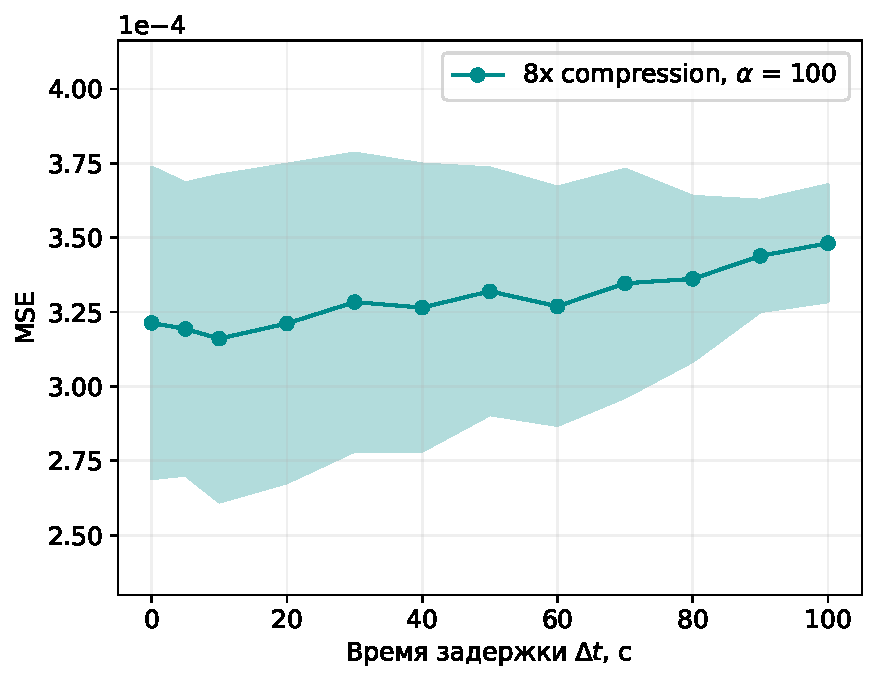
\includegraphics[width=0.65\textwidth]{subs_delta_MSE_dt.pdf}
		\label{fig:3}
	\end{figure}
    Наблюдается характерный минимум при $\Delta t \approx 10 \text{ с}$.
\end{frame}
%----------------------------------------------------------------------------------------------------------
\begin{frame}{Восстановленный снимок}
    Срезы истинного и восстановленного снимков из тестовой выборки.
    Можно наблюдать разность между ними.
    \begin{figure}[h!]
		\centering
		\subfloat[Истинный]{\label{fig:4a}{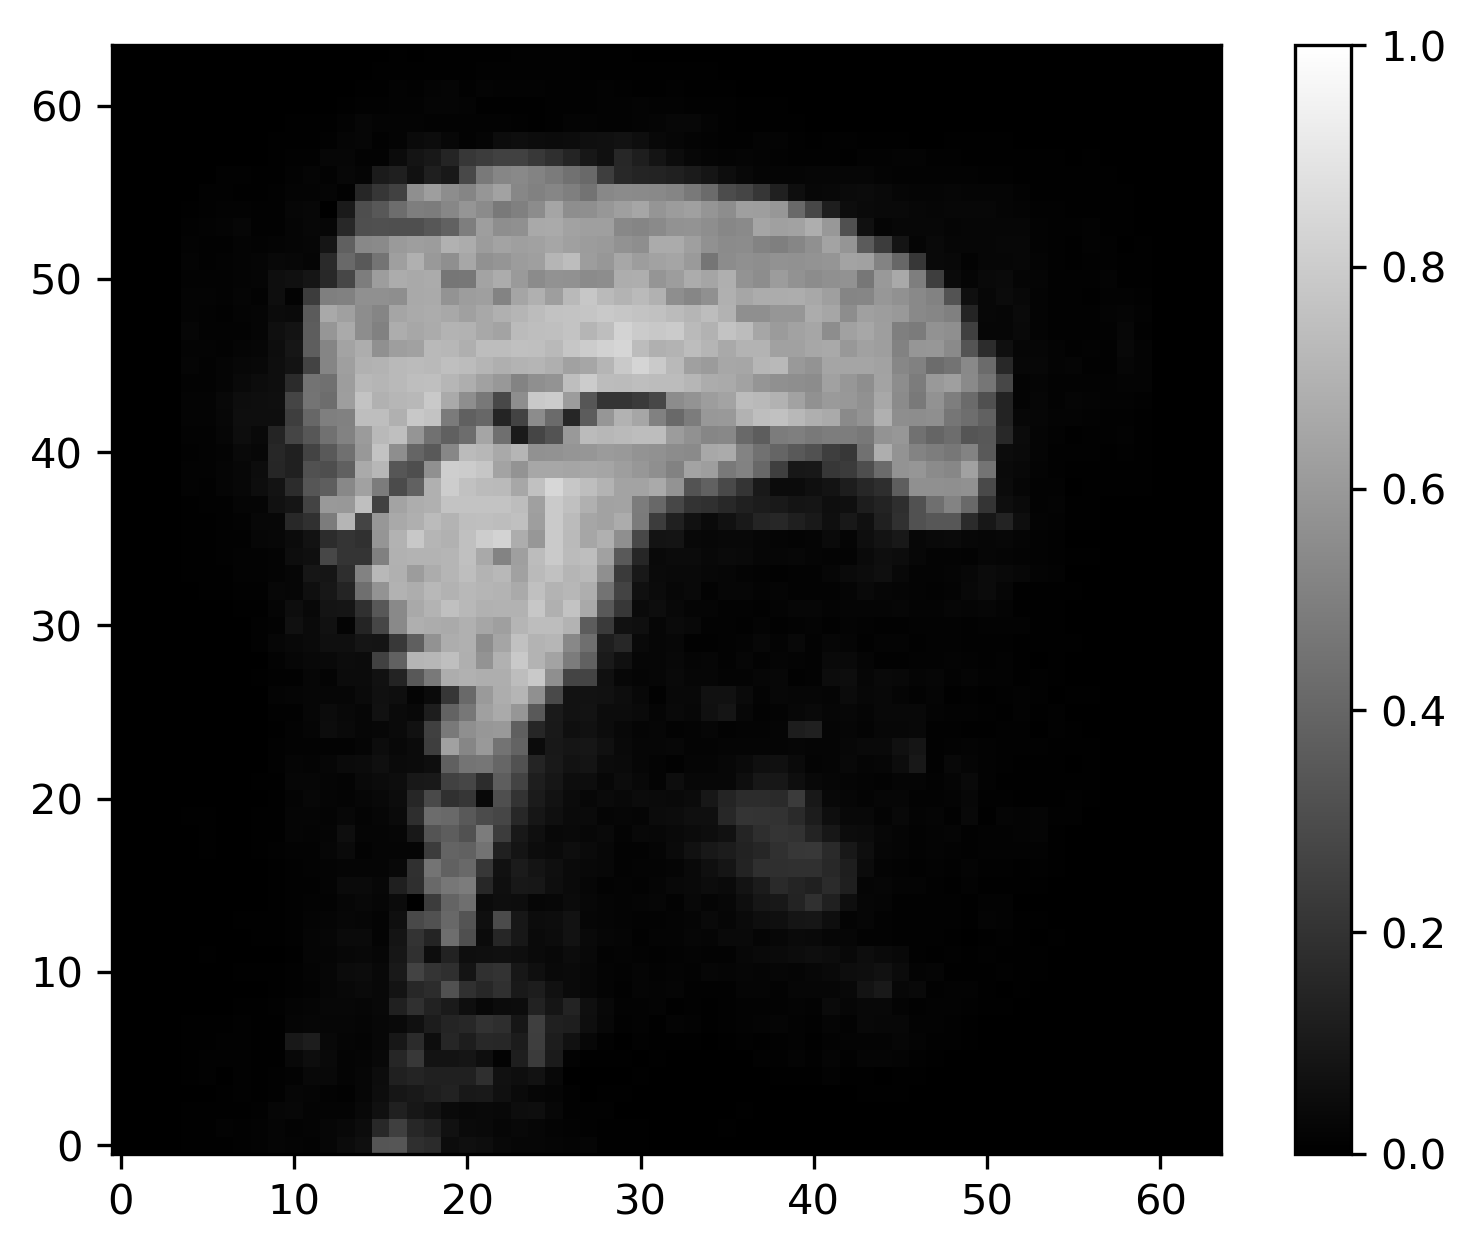
\includegraphics[width=0.33\textwidth]{sub-04-5-1-1000/sub-04-5-1-1000-100-20-_-_-test.png}}}
		\hfill
		\subfloat[Восстановленный]{\label{fig:4b}{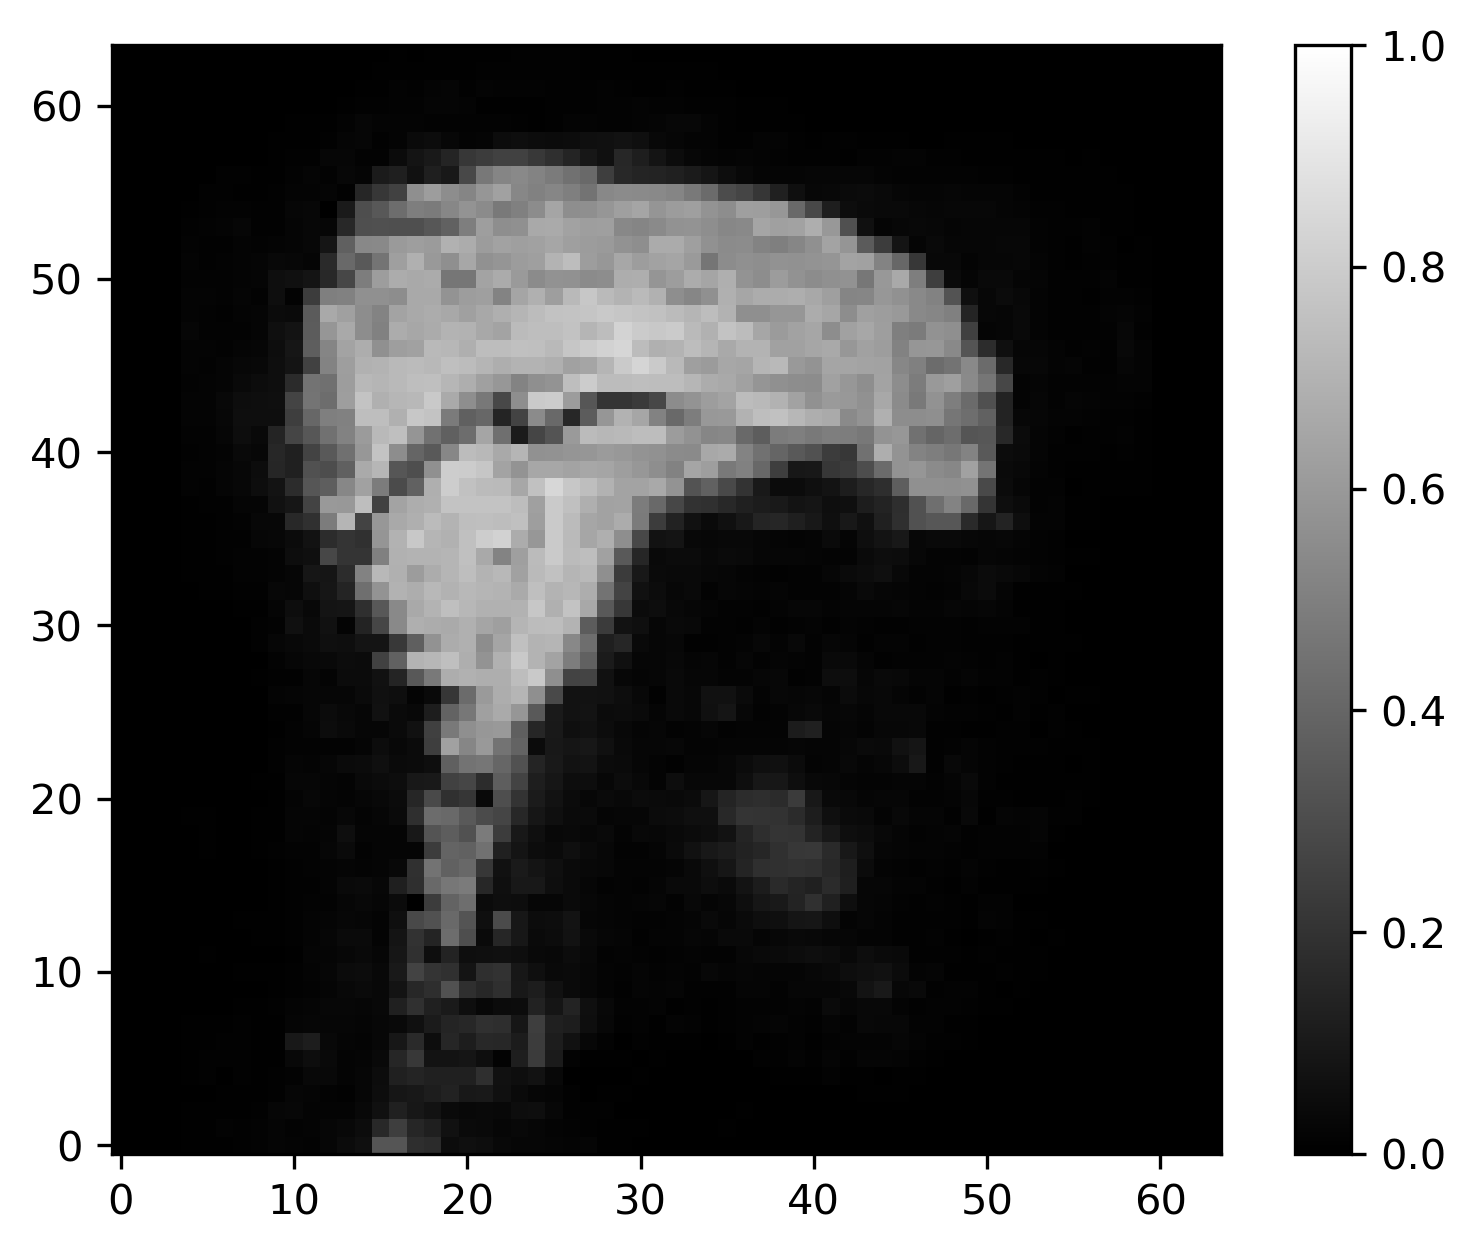
\includegraphics[width=0.33\textwidth]{sub-04-5-1-1000/sub-04-5-1-1000-100-20-_-_-predicted.png}}}
		\hfill
		\subfloat[Разность]{\label{fig:4c}{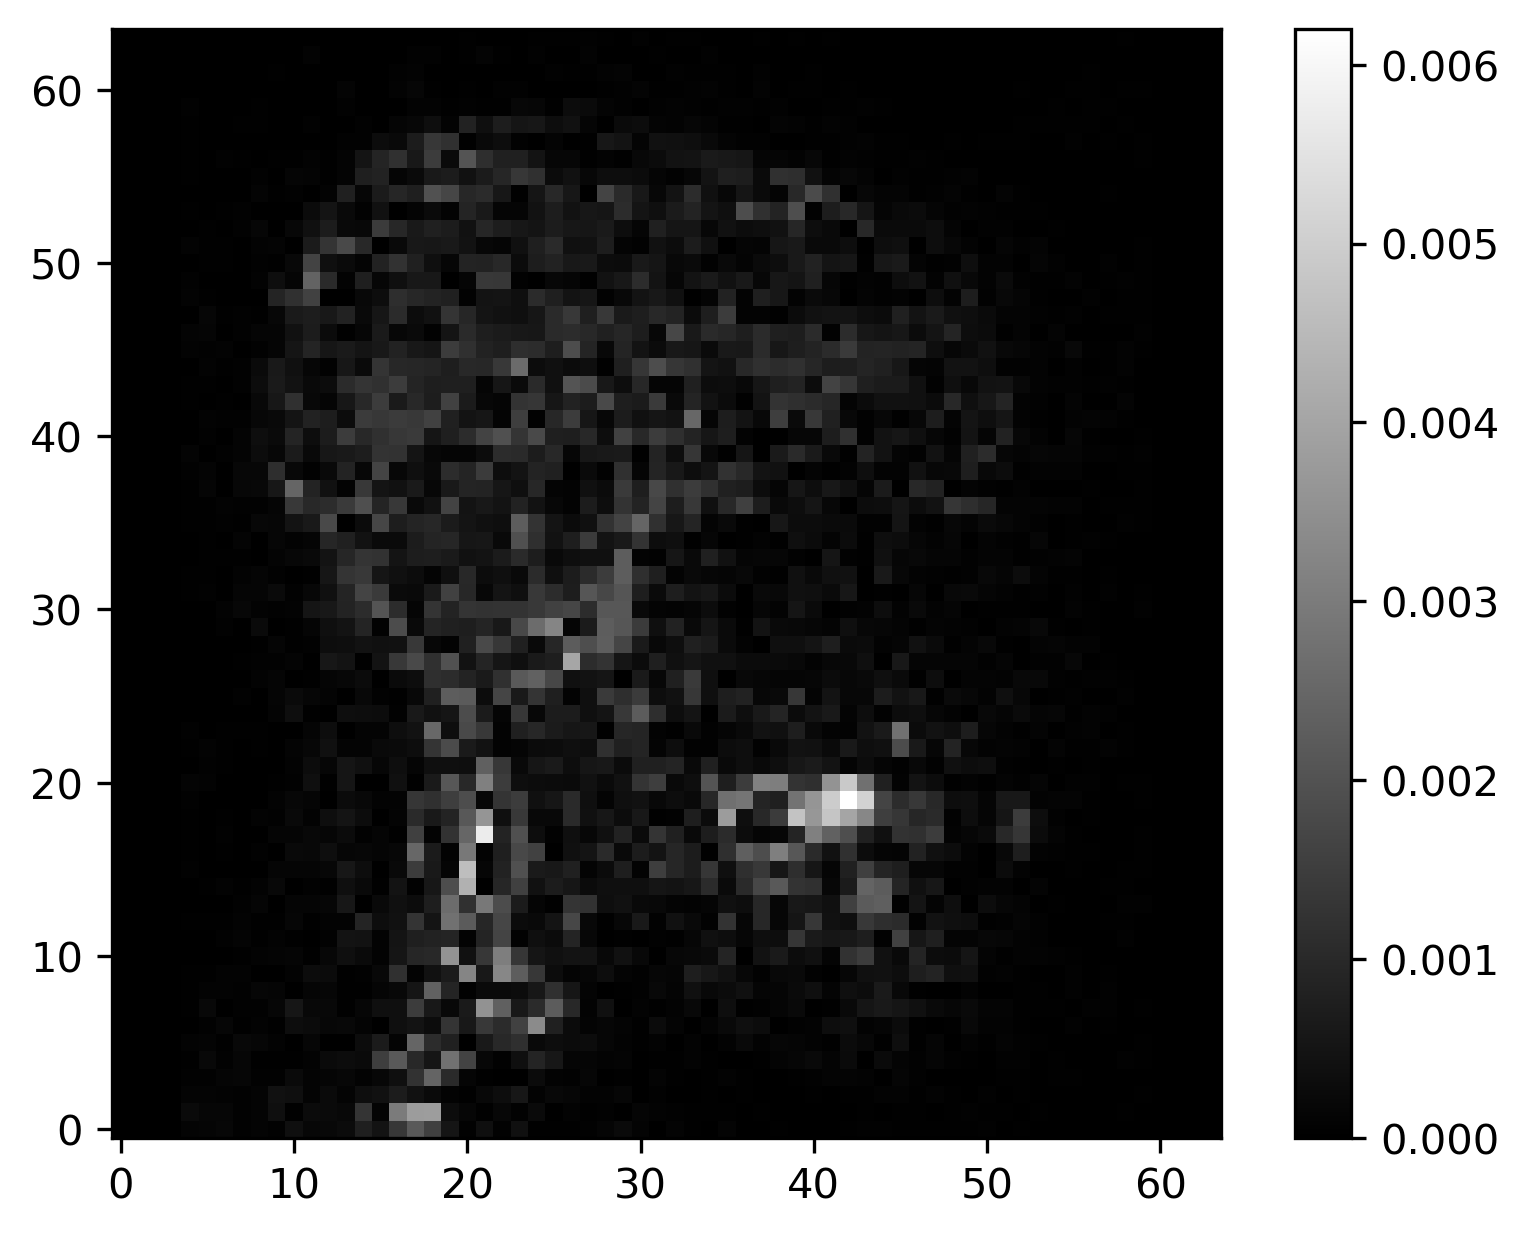
\includegraphics[width=0.33\textwidth]{sub-04-5-1-1000/sub-04-5-1-1000-100-20-_-_-difference.png}}}
		\label{fig:4}
	\end{figure}
    Значения вокселей лежат в отрезке $[0; 1]$, поэтому ошибка порядка $10^{-3} \div 10^{-2}$
    свидетельствует о достаточно точном предсказании.
\end{frame}
%----------------------------------------------------------------------------------------------------------
\begin{frame}{Зависимость от коэффициента регуляризации}
    Зависимость метрики MSE от коэффициента регуляризации $\alpha$.
    Рассматривались коэффициенты сжатия 1, 2, 4 и 8.
    Производилось усреднение по испытуемым.
	Обозначены границы среднеквадратичного отклонения.
    \begin{figure}[h!]
		\centering
		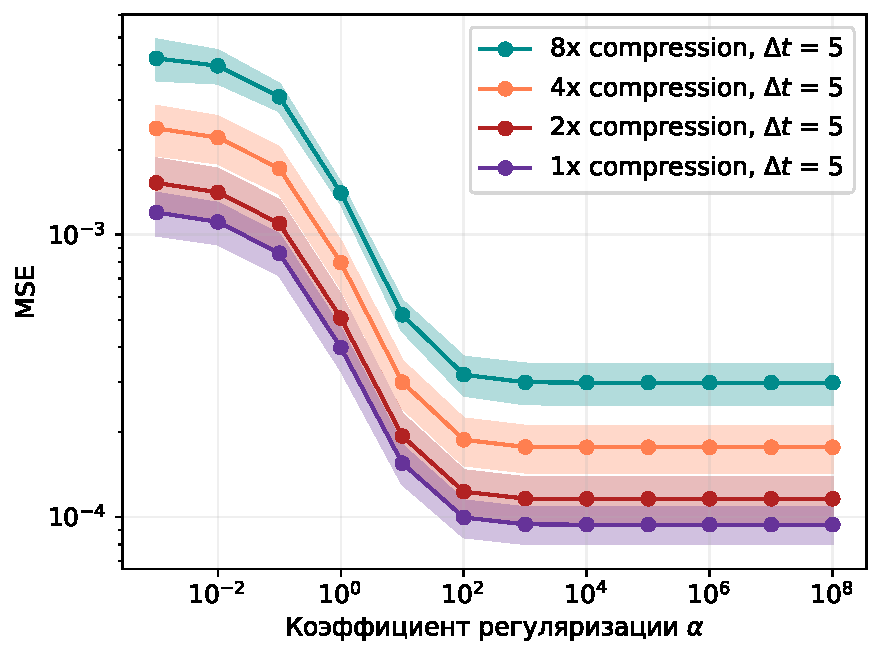
\includegraphics[width=0.65\textwidth]{subs_MSE_alpha.pdf}
		\label{fig:5}
	\end{figure}
    Оптимальное значение коэффициента $\alpha \approx 100$.
\end{frame}
%----------------------------------------------------------------------------------------------------------
\begin{frame}{Распределение весов в среднем по всем вокселям}
    График распределения значений компонент вектора весов модели.
    Производилось усреднение по всем вокселям фиксированного снимка.
    \begin{figure}[h!]
		\centering
		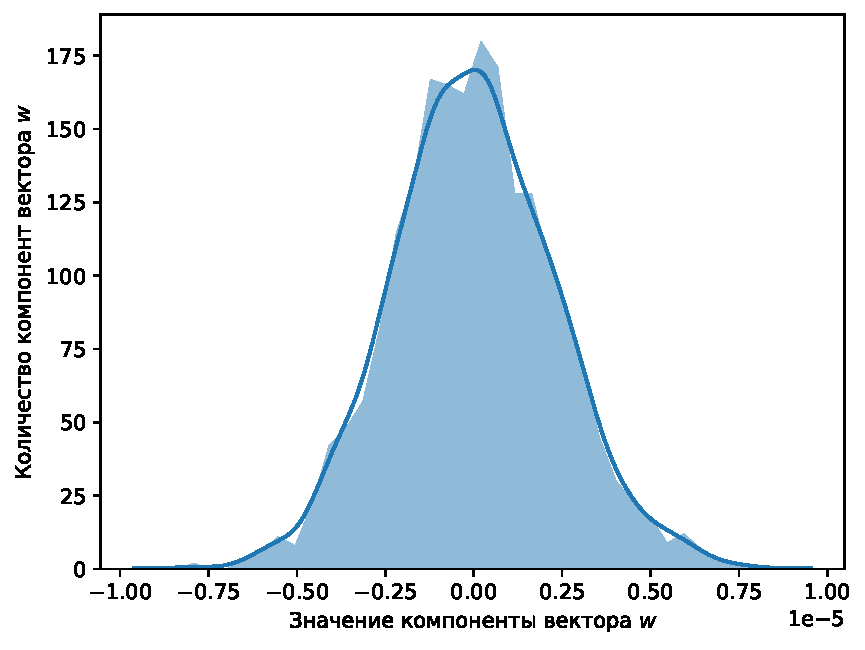
\includegraphics[width=0.65\textwidth]{mean_weight_distribution.pdf}
		\label{fig:6}
	\end{figure}
    Веса модели распределены нормально, а не лежат в окрестности какого-то определенного
    значения.
\end{frame}
%----------------------------------------------------------------------------------------------------------
\begin{frame}{Инвариантность весов относительно человека}
    Проведена проверка гипотезы инвариантности весов модели относительно человека:
	можно ли восстановить снимок фМРТ одного испытуемого, используя
	матрицу весов другого. Использовалась метрика MSE на тестовой выборке.
    \begin{table}[h!]
		\centering
		\begin{tabular}{|c|c|c|}
			\hline
			Матрица весов	&	Истинная	&	Подмешанная\footnotemark[1] \\ \hline \hline
			MSE		& 	$1.02 \cdot 10^{-4}$	 &		$1.05 \cdot 10^{-4}$ \\ \hline
		\end{tabular}
		\label{table:1}
	\end{table}
    Значения MSE практически совпадают. Это свидетельствует о справедливости рассматриваемой гипотезы. 
    \footnotetext[1]{Предсказание снимков одного человека с использованием весов модели другого}
\end{frame}
%----------------------------------------------------------------------------------------------------------
\begin{frame}{Проверка работы на случайном шуме}
    Рассмотрено качество работы метода на случайном шуме. В качестве матрицы $\mathbf{X}$
	взята матрица случайных чисел из $[0; 1]$. Ниже приведены срезы последнего снимка, восстановленного
    последовательно по всем предсказанным изменениям, и значения метрики MSE.
	\begin{figure}[h!]
		\centering
		\subfloat[Истинный]{\label{fig:8a}{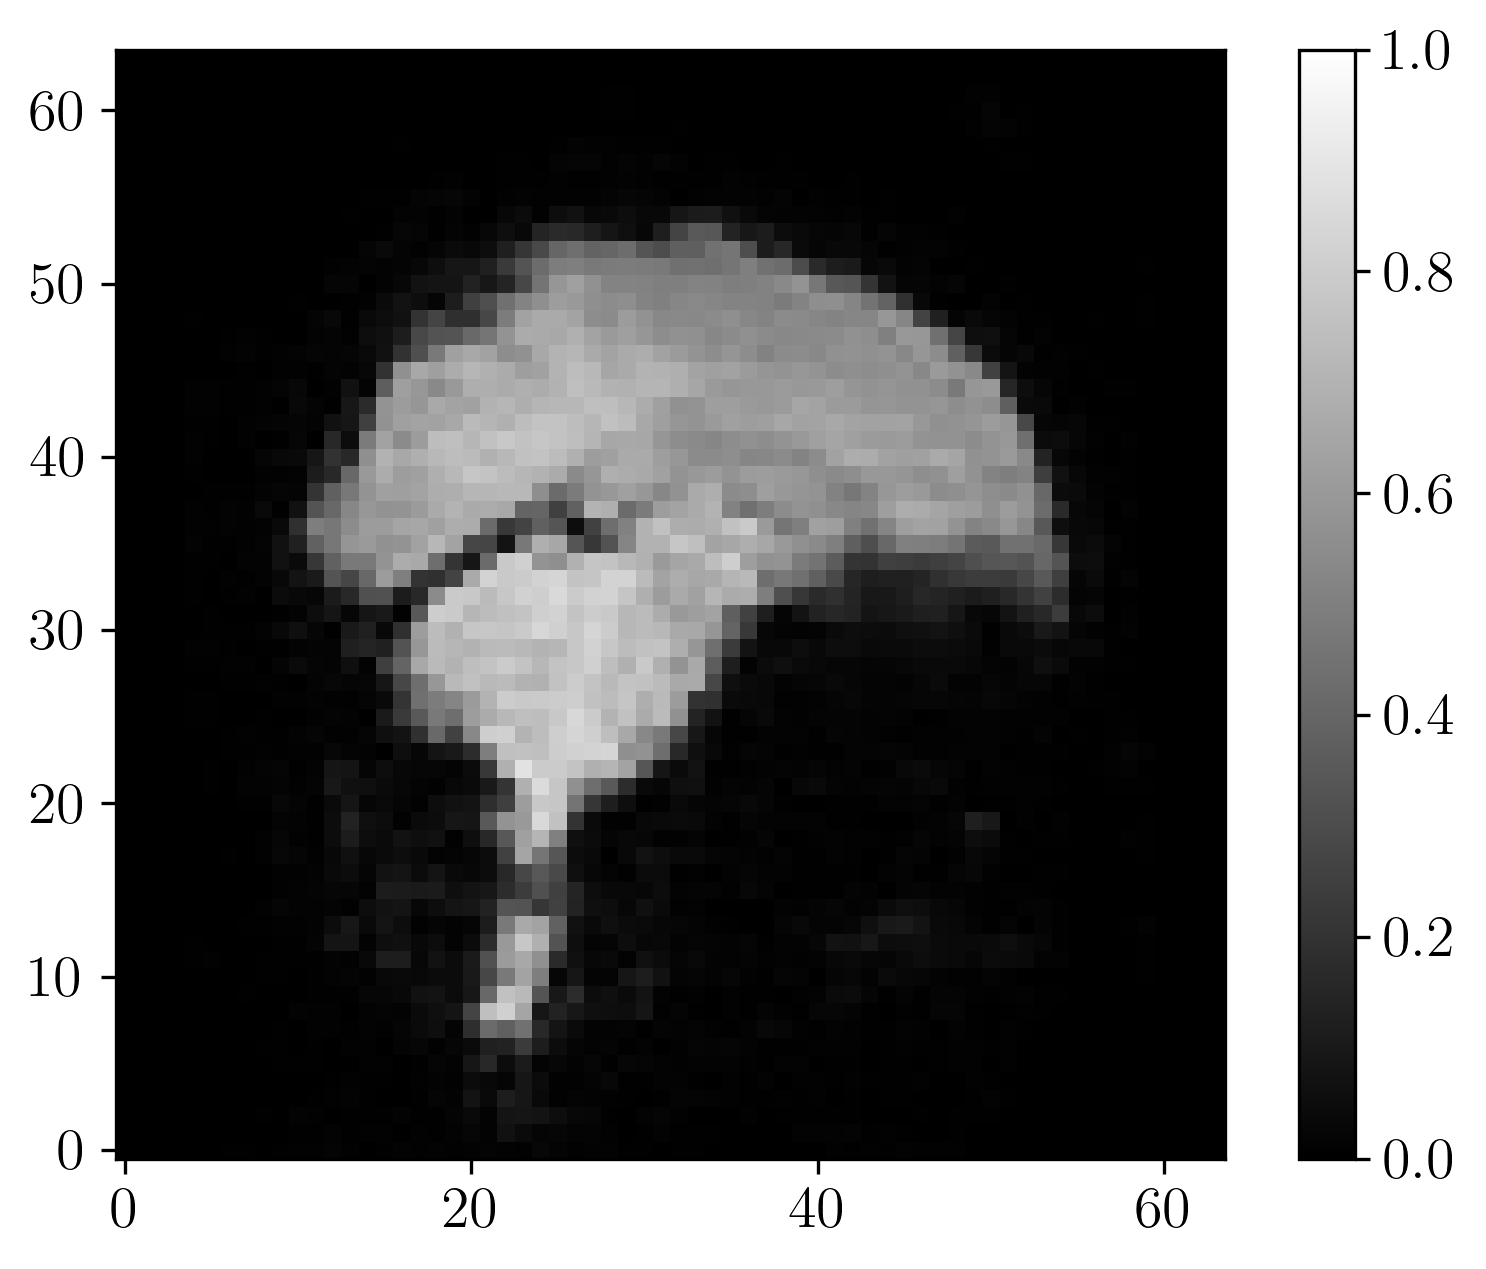
\includegraphics[width=0.33\textwidth]{sub-35-5-1-1000/noised/sub-35-5-1-1000--1-20-_-_-recovered-test.png}}}
		\hfill
		\subfloat[Восстановленный]{\label{fig:8b}{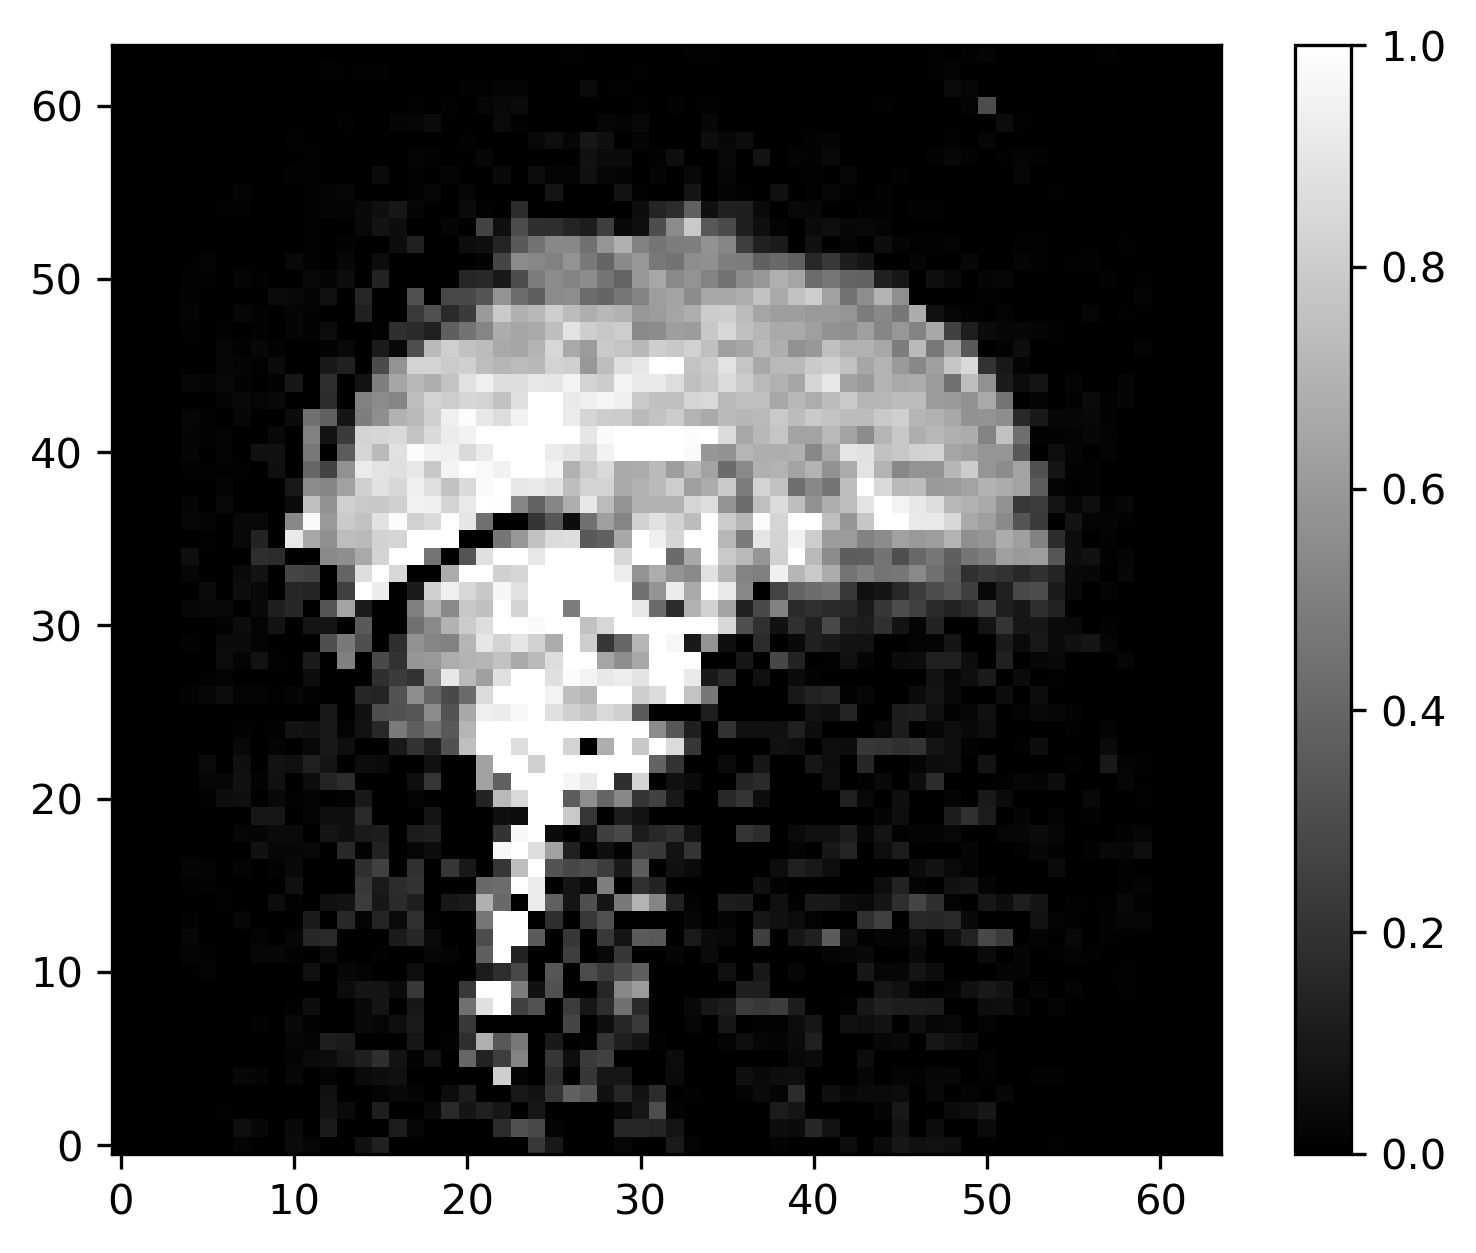
\includegraphics[width=0.33\textwidth]{sub-35-5-1-1000/noised/sub-35-5-1-1000--1-20-_-_-recovered-predicted.png}}}
		\hfill
		\subfloat[Разность]{\label{fig:8c}{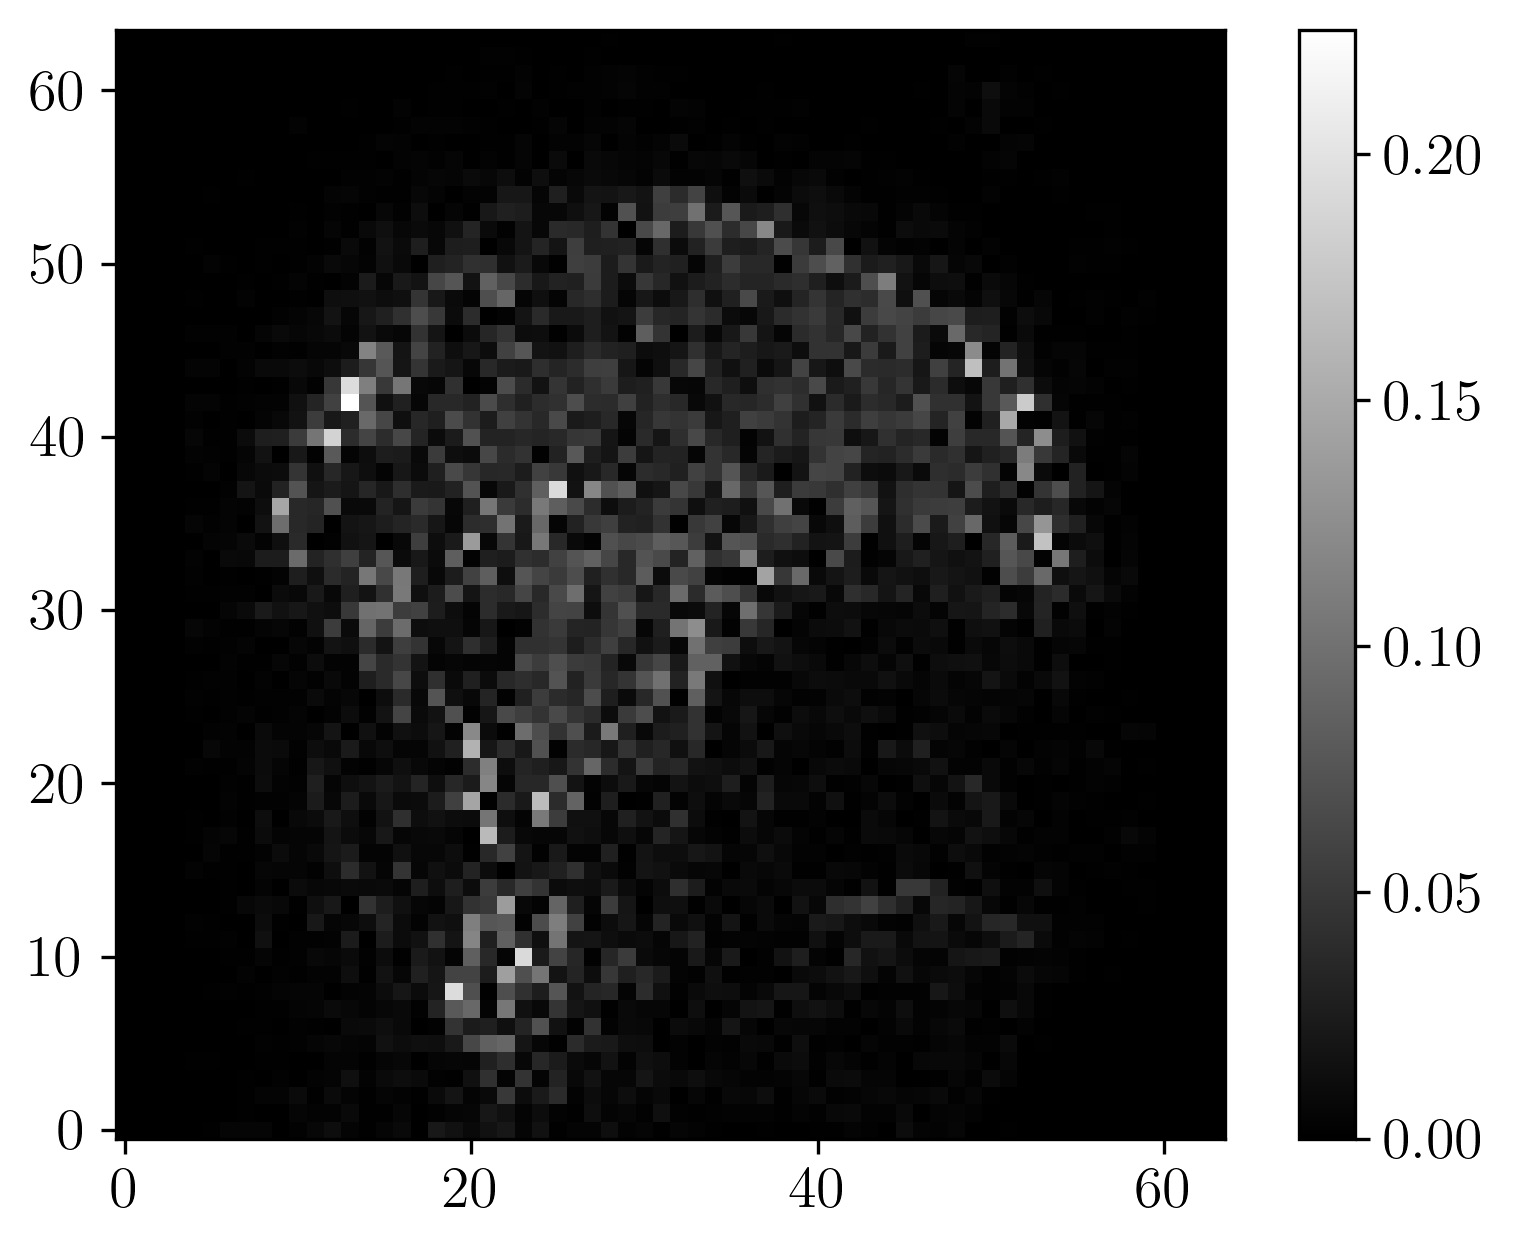
\includegraphics[width=0.33\textwidth]{sub-35-5-1-1000/noised/sub-35-5-1-1000--1-20-_-_-recovered-difference.png}}}
		\label{fig:8}
	\end{figure}
    \begin{table}[h!]
		\centering
		\begin{tabular}{|c|c|c|}
			\hline
			Выборка	&	Истинная	&	Случайный шум \\ \hline \hline
			MSE		& 	$2 \cdot 10^{-3}$	 &		$10^{-1}$ \\ \hline
		\end{tabular}
		\label{table:2}
	\end{table}    
\end{frame}
%----------------------------------------------------------------------------------------------------------
\begin{frame}{Заключение}
    \begin{itemize}
        \item Построен метод аппроксимации последовательности снимков фМРТ по видеоряду,
              просматриваемому человеком.
        \item Справедлива гипотеза о линейной зависимости между данными.
        \item Подтверждена гипотеза о взаимосвязи снимков в последовательности.
        \item Проверена гипотеза инвариантности весов модели относительно человека.
    \end{itemize}
\end{frame}
%----------------------------------------------------------------------------------------------------------
\end{document} 